\chapter{Active Correction as Daemons} \label{cha:opa400}

\clearpage

\section{Introduction}  % =========================================================================

Blaise Thompson extensively discussed multiple forms of active corrections applied to CMDS instruments in Chapter 6 of his dissertation\cite{ThompsonBlaiseJonathan2018a}.
Most prominently, this includes Spectral Delay Correction (SDC).
At the time, active correction for SDC was performed by the orchestration layer, PyCMDS, as the ``autonomic'' system.
The implementation of the autonomic system was tightly coupled to the custom orchstration provided by PyCMDS.
This proved inflexible, and caused the hardware definitions to be intractable in many cases, leading to hard to understand behavior.

When the Wright Group was considering using Bluesky as an orchestration layer, the behavior of the autonomic system was one of the key pieces that made that transition seem hard at first.
There did not seem to be an easy and correct way of inserting the offset logic into the Bluesky Run Engine, as it was implemented for PyCMDS.
Additionally, Bluesky meant separating the behavior as collected, which runs through the Run Engine, from the behavior of hardware in an interactive session, as when attempting to initially find signal.
Upon reflecting, and taking a step back to consider the desired outcome, the solution became obvious: instead of inserting this logic as a modifier to the Run Engine, that logic can be implemented as a daemon which wraps the hardware daemon.
This intermediate daemon provides the controls of offsets being applied or ignored.
Additionally, daemons can be more specialized to the particular task, and thus are easier to use and describe compared to the general purpose autonomic system of PyCMDS.
To the client program, whether that is an interactive client like \yaqcqtpy{} or the Bluesky Run Engine, this daemon looks and acts like a simple motor that gets told to go to a particular position and does so.

Herein, we will look at two instances of active correction as daemons.
First, SDC itself and the \texttt{attune-delay} daemon which implements it.
And second, the \texttt{ndinterp} daemon which allows for more complicated relationships among controlling hardware.

\clearpage

\section{attune-delay}  % =============================================================

Spectral delay occurs largely due to transmissive optics which have a wavelength-dependent index of refraction and changes of the optical path length within the tunable light sources.
When pulses are less a picosecond long (or even shorter), even small variations will cause overlap in time to diminish rapidly.
Spectral Delay Correction (SDC) is an active correction technique which employs the delay motors already included in the instrument to adjust the path length of each beamline to account for any variation in arrival time as a function of wavelength.

SDC ``curves'' are represented as Attune \texttt{Instrument} objects.
This allows reuse of utilities that were used for OPA tuning curves previously.
For an OPA \texttt{Instrument} object, the whole thing represents one light source, each \texttt{Arrangement} represents one configuration of motors to produce a unique range of light, and each \texttt{Tune} represents the mapping of a single motor position (or another \texttt{Arrangement}) from the input color.
In contrast, for an SDC \texttt{Instrument} object, the levels are all shifted one down: the light source \texttt{Instrument} keys are the \texttt{Arrangement} keys of the SDC curve, and the \texttt{Arrangement} keys from the light sources are the \texttt{Tune} keys.
The \texttt{Tune} outputs are not motor positions directly, but rather offset in picoseconds for the particular light source using the particular \texttt{Arrangement}.
This allows a single \texttt{Instrument} to fully describe all possible required offsets for a laser system which may use multiple \texttt{Arrangement}s to do experiments.
The total offset is the sum of all offsets from each light source.

The objective is to create a daemon which performs the necessary offset.
Such a daemon will wrap a daemon for a translation stage, but can also perform the logical transform from displacement in length units to displacement in time units from some arbitrary zero mark which can be configured.
The offset will change whenever one of the values used to compute it changes: either a light source changes color or \texttt{Arrangement}.
When creating a daemon to compute and control the delay and offset, there is a natural inclination to have this daemon be a client of the light source and simply call for the color of the light source every time it computes the offset.
The problem with this is that the daemon has no way to tell that the color of a light source has changed.
To remedy this, a delay offset computing daemon would have to poll each light source for their position so that it could react as it needs to.
This tight polling is expensive, and requires balancing polling rate and responsiveness.
Additionally, when the light source changes color, it is possible that the delay will be the slowest motor, and so any client program will want the light source to remain busy until the associated delay is done moving.
All of these factors combined mean that instead, the Attune daemon which controls the light sources must be a client of the Attune Delay offsetting daemon.
The Attune Delay daemon simply caches the position and active arrangement of each controlling hardware and uses that cache to compute offsets.
It must recompute and reapply the offset whenever any controlling light source moves.
The Attune daemon can poll its associated delays for busy status whenever it moves, maintaining its own busy state that a client might be polling.
The client-daemon relationships are summarized in Figure \ref{act_corr:fig:attune_delay_flow}

\begin{figure}
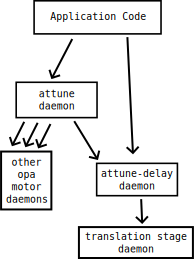
\includegraphics[width=5in]{active_correction/images/attune_delay_flow}
\caption[Attune Delay Information Flow]{The relationships between clients and daemons with an Attune Delay daemon.}
\label{act_corr:fig:attune_delay_flow}
\end{figure}

To make this work, the Attune Delay daemon exposes a set of messages that the light source Attune daemon can call to communicate changes.
Specifically, \texttt{set\_control\_tune} and \texttt{set\_control\_position} are called by the light source daemon at initialization and whenever the active arrangement or position, respectively, are changed.
When the Delay daemon receives these calls, it will recompute and reapply the offset.
The former accepts a string for the control key, i.e. the name of the light source daemon, and a string for the tune, which is the arrangement of the light source.
The latter similarly accepts the control key and a double precision floating point position.
Those are the only two messages that are used by the Attune daemon.

In addition, there are messages used by engineering interfaces or specialized clients to control the behavior of the Attune Delay daemon.
\texttt{set\_control\_active} allows for selectively turning off offsets from each light source.
This is useful for collecting the SDC offset curves themselves, which are typically collected without active correction applied to avoid needing to add two corrections together.
The position and tune caches are updated even if the controlling hardware is inactive.
This allows the correct offset to be applied if the hardware is toggled to active.
\texttt{set\_zero\_position} takes a position in the coordinates of the underlying translation stage and calls that position "zero" for the logical delay.
\texttt{set\_instrument} allows overwriting of the entire \texttt{Instrument} object.
This is used by data processing scripts to apply newly collected SDC curves.
The \texttt{Instrument} is stored in the Attune Store, where it can be reloaded.
Client connections are interrupted so that they are aware that assumptions about the applied \texttt{Instrument} are broken and they must refresh their cached copies.

Each of the setting methods mentioned above have associated methods for retrieving the information, as well as methods to get related quantities such as limits or units.

In all, the Attune Delay daemon looks just like any other \yaq{} daemon to a client program which does not require knowledge of the details of the offsetting behavior.
While all of the information is available to clients, if one wishes to do a simple one dimensional scan, it behaves just as any other motor.
Its only functional difference in that regard from the underlying translation stage is that the units and zero position are changed to represent the logical behavior of the stage as part of a larger instrument rather than the physical behavior of the stage alone.

\clearpage

\section{ndinterp}  % ===================================================================


Phase matching is an important factor contributing to the constructive interference of non-linear mixing processes. 
Some mixing processes cannot be phase matched, and therefore have destructive interference which causes diminished signal with increased path length.
To properly account for phase matching, relative angles of beam propagation combined with the energies and indices of refraction for each incident beam and the generated output beam must be taken into account.
Since it is wavelength dependent, a desired experiment may span a region where the optimal phase matching requires incoming light at significantly differing angles.
The Wright Group, and in particular Emily Kaufman, have been attempting to actively correct for angle of incidence to ensure proper phase matching for all wavelengths of a desired experiment.
To accomplish this task, the idea is to move the retroreflector laterally to displace the beam horizontally while maintaining the output angle from the retroreflector.
The beam will therefore hit a different position on the focusing optic.
The focussing optic will maintain focus for the parallel incoming beams to the same spot on the sample, but with differing angles.\footnote{This is technically only true for parabolic mirrors, but in practice is often a good enough approximation for spherical mirrors used approximately on axis}
Depending on the free aperture of the mirrors and the focal length of the focussing optic, this can provide several degrees of available offset while maintaining spatial overlap at the sample.
Figure \ref{act_corr:fig:phase_matching_angle} shows the effect of translating a retroreflector as described above.
This figure is not to scale, simply a cartoon illustrating the principle.
The ideal angle can be calculated, but is dependent on multiple laser colors in complicated ways.
Unlike SDC, phase matching corrections are not separable for each light source and additive.

\begin{figure}
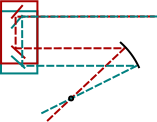
\includegraphics[width=5in]{active_correction/images/phase_matching_angle}
\caption[Phase Matching Angle]{The same incident beam angle will be translated if the retroreflector is translated.
A focussing optic causes the beams to converge to the same location in space but at different angles.}
\label{act_corr:fig:phase_matching_angle}
\end{figure}

The hardware required for active phase matching is a translation stage mounted perpendicular to the beam path with a retroreflector.
Because a retroreflector is already required for delays, this lateral translation stage is mounted on top of the delay
This does require some tight consideration for physical size of the translation stage, as it must both support the mass of the retroreflector and be short enough for mirrors to sit on top.

For this process, the information required is almost precisely the same as the Attune Delay daemon detailed above.
So, to accomplish the task, we must implement a daemon that looks to the light source Attune daemon exactly like an Attune Delay daemon.
This is not strictly required for this daemon specifically, but does allow it to be quickly implemented without changing existing daemons.
The daemon must be notified of when controlling hardware changes position and recompute its offsets.
This daemon, called NDInterp, performs N-Dimensional interpolation to be a maximally flexible active correction daemon.
However, the \texttt{Tune} information is not used, so a method which does nothing is provided so that the calling client daemon does not have to be changed. 
Instead of being backed by an Attune \texttt{Instrument} which accepts independent offsets which are additive, a single multidimensional offset is used.
This multidimensional offset is represented as a WrightTools Data file.
The data file is configured to have a single \texttt{WrightTools.Data} object which has axes of the control hardware and a channel which represents the required offset.
implement a daemon that looks to the opa exactly like an attune-delay
Similar to Attune Delay, NDInterp has a zero position from which all offsets are relative.

Since the offset is fundamentally multidimensional, independent control hardware cannot be toggled on and off like they can for the Delay daemon.
Instead, there is a single boolean \yaq{} property which can disable the offset behavior entirely to allow for experiments which do not require the active phase matching.

This approach to active phase matching allowed us to quickly and easily write a daemon that is capable of performing the active correction required.

\clearpage
